\documentclass[preview=true]{standalone}
\usepackage{tikz}
\usepackage{pgfplots}
\usepackage[siunitx, american]{circuitikz}
\usepackage[utf8]{inputenc}
\usepackage{newtxtext,newtxmath}
\usepackage[T1]{fontenc}
\pgfplotsset{compat=1.18}
\usepgfplotslibrary{units, fillbetween, smithchart, colormaps}
\usetikzlibrary{positioning, shapes, arrows, arrows.meta, graphs, shapes.geometric, math}
\tikzset{>=latex} % Better arrow tips

\begin{document}
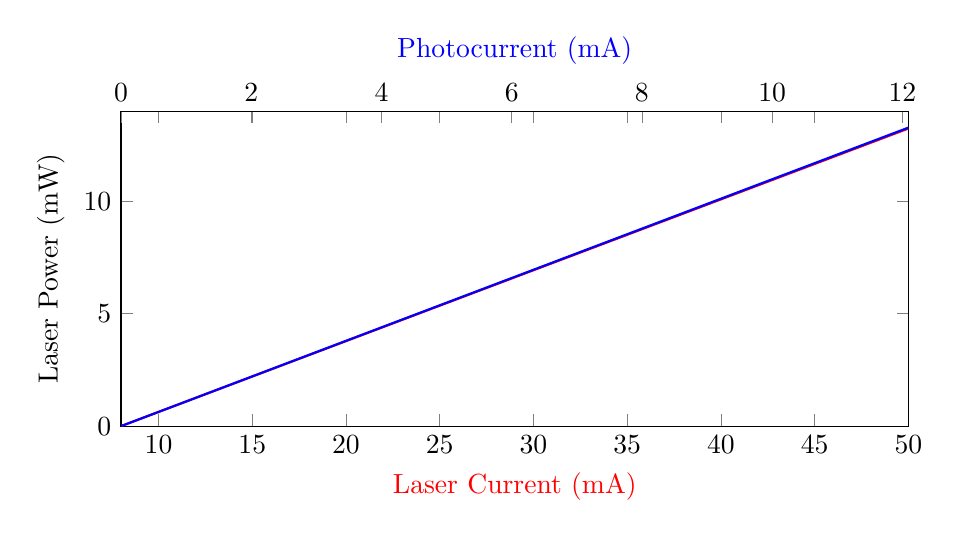
\begin{tikzpicture}
\begin{axis}[width={10cm}, height={4cm}, scale only axis, xlabel={Laser Current (mA)}, ylabel={Laser Power (mW)}, ymin={0}, ymax={14}, xmin={8}, xmax={50}, xlabel style={red},]
    \addplot[no marks, thick, color={red}]
        coordinates {
            (-0.0,0)
            (1.0,0)
            (2.0,0)
            (3.0,0)
            (4.0,0)
            (5.0,0)
            (6.0,0)
            (7.0,0)
            (8.0,0.0)
            (9.000000000000002,0.3150000000000003)
            (10.0,0.63)
            (11.0,0.9449999999999997)
            (12.0,1.26)
            (13.000000000000002,1.5750000000000002)
            (14.0,1.89)
            (15.0,2.205)
            (16.0,2.52)
            (17.0,2.8350000000000004)
            (18.000000000000004,3.1500000000000004)
            (19.0,3.465)
            (20.0,3.78)
            (21.0,4.095000000000001)
            (22.0,4.41)
            (23.0,4.725)
            (24.0,5.04)
            (25.0,5.355)
            (26.000000000000004,5.670000000000001)
            (27.0,5.984999999999999)
            (28.0,6.3)
            (29.0,6.615)
            (30.0,6.93)
            (31.0,7.245)
            (32.0,7.56)
            (33.0,7.875)
            (34.0,8.190000000000001)
            (35.0,8.505)
            (36.00000000000001,8.820000000000002)
            (37.0,9.135)
            (38.0,9.45)
            (39.0,9.764999999999999)
            (40.0,10.08)
            (41.0,10.395)
            (42.0,10.71)
            (43.0,11.025000000000002)
            (44.0,11.34)
            (45.0,11.655)
            (46.0,11.969999999999999)
            (47.0,12.285)
            (48.0,12.6)
            (49.0,12.915000000000001)
            (50.0,13.23)
        }
        ;
\end{axis}
\begin{axis}[width={10cm}, height={4cm}, scale only axis, xlabel={Photocurrent (mA)}, ylabel={Laser Power (mW)}, ymin={0}, ymax={14}, xmin={0}, xmax={12.09334},      axis y line*=right, axis x line*=top, xlabel style={blue},axis y line=none]
    \addplot[no marks, thick, color={blue},]
        coordinates {
            (5.651475e-5,6.20087228439763e-5)
            (0.000251357,0.0002757921878428791)
            (0.0006014396,0.000659907395216151)
            (0.001056724,0.00115945139346061)
            (0.001769435,0.0019414472240509109)
            (0.002965913,0.0032542385341233267)
            (0.00467636,0.005130963353083169)
            (0.007549197,0.008283077682685977)
            (0.01634339,0.017932181259600614)
            (0.2881295,0.31613945578231295)
            (0.580155,0.6365536537195523)
            (0.8756634,0.9607893350888743)
            (1.164539,1.277747421549265)
            (1.456461,1.5980480579328507)
            (1.748156,1.9180996269475532)
            (2.0396099999999997,2.2378867676102696)
            (2.331031,2.557637700241387)
            (2.622013,2.8769069563309193)
            (2.913249,3.1964549045424624)
            (3.204362,3.5158678955453153)
            (3.495431,3.835232609172701)
            (3.786039,4.1540915075707705)
            (4.076237,4.47250054860654)
            (4.366104,4.790546412113232)
            (4.655776,5.108378319069564)
            (4.944829,5.42553105113013)
            (5.233424,5.742181259600615)
            (5.521758,6.058545095457538)
            (5.810138,6.374959403116085)
            (6.097754,6.690535439982446)
            (6.385664,7.006434057493966)
            (6.673594,7.322354619267061)
            (6.961834,7.6386153170945805)
            (7.2499,7.954685099846391)
            (7.537446,8.270184331797235)
            (7.824822999999999,8.585498134737767)
            (8.111843,8.900420232609175)
            (8.39823,9.214647794601712)
            (8.684035999999999,9.528237875795478)
            (8.969541,9.841497695852535)
            (9.2547,10.154377880184331)
            (9.539503,10.466867456660083)
            (9.825405,10.780562870309415)
            (10.111270000000001,11.094217687074831)
            (10.39711,11.407845073513275)
            (10.68193,11.720353302611366)
            (10.96642,12.032499451393459)
            (11.249820000000001,12.343449637919685)
            (11.53181,12.652852754004828)
            (11.812990000000001,12.96136712749616)
            (12.09334,13.268970814132103)
        }
        ;
\end{axis}
\end{tikzpicture}
\end{document}